\section{Android Open ADK}
\label{adk_sec}

The iNEMO board and the Android-powered device communicate on a USB bus. USB is an asymmetric protocol in that one participant acts as a USB Host and all other participants are USB Devices. The USB Host has two important tasks. The first is to be the bus master and control which device sends data at what times. The second key task is to provide power, since USB is a powered bus (see {\bf Figure \ref{fig:usb_normal}}). The problem with supporting accessories on Android in the traditional way is that relatively few devices support Host mode. Android Open ADK offers an answer to this problem, inverting the normal USB relationship.

\begin{center}
	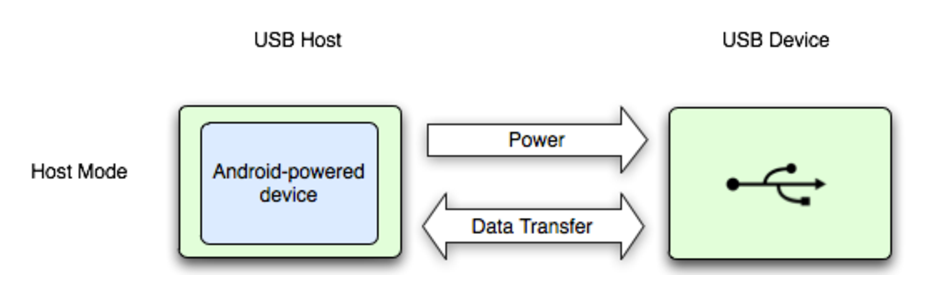
\includegraphics[width=1\linewidth]{pics/usb_normal.eps}
	\captionof{figure}{Normal USB relationship.}
	\label{fig:usb_normal}
\end{center}

During the Google I/O 2011 conference, Google announced the Android Open Accessory APIs for Android. These APIs allow USB accessories to connect to Android devices running Android 3.1 or Android 2.3.4 without special licensing or fees. The new ``accessory mode'' does not require the Android device to support USB Host mode. In accessory mode the Android phone or tablet acts as the USB Device and the accessory acts as the USB Host. This means that the accessory is the bus master and provides power (see {\bf Figure \ref{fig:usb_accessory}}).

\begin{center}
	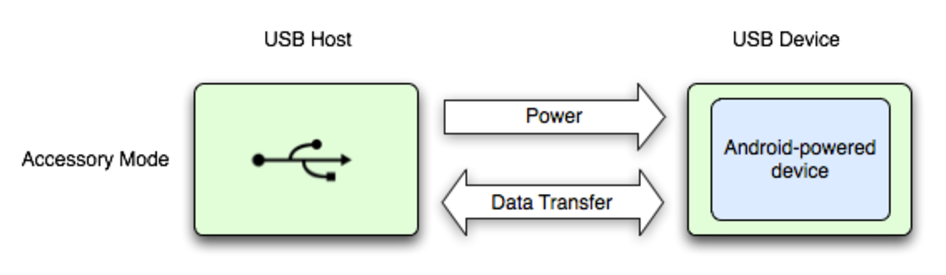
\includegraphics[width=1\linewidth]{pics/usb_accessory.eps}
	\captionof{figure}{Inverted USB relationship: the accessory acts as the USB host.}
	\label{fig:usb_accessory}
\end{center}

Building an Open Accessory is quite simple, as the only HW requirements are to include a USB host and provide power to the Android device. The accessory needs to implement a simple handshake to establish a bi-directional connection with an application running on the Android device.

The handshake starts when the accessory detects that a device has been connected to it. The Android device will identify itself with the VID/PID that are defined by the manufacturer and the model of the device. The accessory then sends a control transaction to the Android device asking if it supports accessory mode.

Once the accessory confirms the Android device supports accessory mode, it sends a series of strings to the Android device using control transactions. These strings allow the Android device to identify compatible applications as well as provide a URL that Android will use if a suitable app is not found. Next the accessory sends a control transaction to the Android device telling it to enter accessory mode.

The Android device then drops off the bus and reappears with a new VID/PID combination. The new VID/PID corresponds to a device in accessory mode, which is Google's VID 0x18D1, and PID 0x2D01 or 0x2D00. Once an appropriate application is started on the Android side, the accessory can now communicate with it using the first Bulk IN and Bulk OUT endpoints.

The protocol is quite easy to implement on the accessory: a complete tutorial on the implementation of Open ADK can be found in the USB section of the official Android Developer's Guide\footnote{Android Developer's Guide: \url{http://developer.android.com/guide/index.html}}.

